\documentclass[nobib]{tufte-handout}
% \documentclass[fleqn,reqno,12pt]{article}

%========================================
% Packages
%========================================

\usepackage[nographicx, nohyperref, nosubcaption, nogb4e]{mfpackages}
\usepackage{mfenvironments}
\usepackage{mfcommands}
% for info boxes
\usepackage{newfloat, caption}
\DeclareCaptionType{InfoBox}


%========================================
% Bibliography
%========================================

\bibliography{references.bib}

%========================================
% General Layout Tweaks
%========================================

% \usepackage[margin=2cm]{geometry}

% Itemize
\renewcommand{\labelitemi}{\large{$\mathbf{\cdot}$}}    % itemize symbols
\renewcommand{\labelitemii}{\large{$\mathbf{\cdot}$}}
\renewcommand{\labelitemiii}{\large{$\mathbf{\cdot}$}}
\renewcommand{\labelitemiv}{\large{$\mathbf{\cdot}$}}
% Description
\renewcommand{\descriptionlabel}[1]{\hspace\labelsep\textsc{#1}}

% Figure Captions
\usepackage{caption} % use corresponding myfiguresize!
\setlength{\captionmargin}{20pt}
\renewcommand{\captionfont}{\small}
\setlength{\belowcaptionskip}{7pt} % standard is 0pt

%========================================
% Define colors and comment functions
%========================================

\usepackage{xcolor}
\definecolor{firebrick}{RGB}{178,34,34}
\definecolor{DarkGreen}{RGB}{34,178,34} 
\definecolor{DarkOrange}{RGB}{255,100,50}
\renewcommand{\mf}[1]{\textcolor{firebrick}{[mf: #1]}}  
\newcommand{\tr}[1]{\textcolor{DarkOrange}{[tr: #1]}}  
%========================================
% Configuring the R code presentation
%========================================

\usepackage{courier}
\usepackage{listings}
\usepackage{color}
% the following defines the layout for the R code
\lstset{ %
  language=R,                     % the language of the code
  basicstyle=\footnotesize\ttfamily, % size and type of the fonts that are used for the code
  numbers=left,                   % where to put the line-numbers
  numberstyle=\tiny\color{gray},  % the style that is used for the line-numbers
  stepnumber=1,                   % the step between two line-numbers. If it's 1, each line
                                  % will be numbered
  numbersep=5pt,                  % how far the line-numbers are from the code
  backgroundcolor=\color{white},  % choose the background color. You must add \usepackage{color}
  showspaces=false,               % show spaces adding particular underscores
  showstringspaces=false,         % underline spaces within strings
  showtabs=false,                 % show tabs within strings adding particular underscores
  frame=single,                   % adds a frame around the code
  rulecolor=\color{white},        % if not set, the frame-color may be changed on line-breaks within not-black text (e.g. commens (green here))
  tabsize=2,                      % sets default tabsize to 2 spaces
  captionpos=b,                   % sets the caption-position to bottom
  breaklines=true,                % sets automatic line breaking
  breakatwhitespace=false,        % sets if automatic breaks should only happen at whitespace
  title=\lstname,                 % show the filename of files included with \lstinputlisting;
                                  % also try caption instead of title
  keywordstyle=\color{blue},      % keyword style
  commentstyle=\color{DarkGreen}, % comment style
  stringstyle=\color{DarkOrange}, % string literal style
  escapeinside={\%*}{*)},         % if you want to add a comment within your code
  morekeywords={*, ...}            % if you want to add more keywords to the set
}


% this is for showing the R output
\lstnewenvironment{rc}[1][]{\lstset{language=R}}{}

% this is for inline R code
\newcommand{\ri}[1]{\lstinline{#1}}  %% Short for 'R inline'


%========================================
% Article Header 
%========================================


\title{Bayesian regression modeling for (factorial designs): A tutorial}
\author{Michael Franke \& Timo Roettger}
\date{}

%========================================
% Article Body
%========================================

\begin{document}
\maketitle

\begin{abstract}
  \noindent Generalized linear mixed models are very well-rounded and handy tools for statistical inference. Bayesian approaches to applying these models have recently become increasingly popular. This tutorial provides an accessible, non-technical introduction to the use and feel of Bayesian mixed effects regression models. The focus is on data from a factorial-design experiment. \\
  
  \medskip
  
  \noindent \textbf{This tutorial should take you about 1 hour.}
\end{abstract}

\section{Motivation \& intended audience}

This tutorial provides a very basic introduction to Bayesian regression modeling using R \citep{Manual}. We wrote this tutorial with a particular reader in mind. If you have used R before and if you have a basic understanding of linear regression, and now you want to find out what a Bayesian approach has to offer, this tutorial is for you. In comparison to other introductions \citep[e.g.][]{SorensenHohensteinb2016:Bayesian-linear}, this tutorial remains very conceptual. We don’t want to ``sell Bayes'' to you, and we do not want to scare you away with mathematical details. We just want to give you an impression of how a Bayesian regression analysis looks and feels. So no reason to be afraid! But also: no reason to be bored, because we \emph{will} cover all the essential concepts and we \emph{will} explain how to run and interpret the output of a Bayesian regression analysis using the wonderful R package \texttt{brms} written by Paul \citet{buerkner2016brms}.

If you don’t have any experience with regression modeling, you will probably still be able to follow, but you might also want to consider doing a crash course. To bring you up to speed, we recommend the excellent two-part tutorial by Bodo \citet{Winter2013:Linear-models-a} on mixed effects regression in a non-Bayesian ---a.k.a.~classical or frequentist--- paradigm. In a sense, this tutorial could be considered part three of Bodo's nice and lofty introduction. We will for example use the same data set.

This tutorial contains text boxes (with a gray background) which contain additional background information on some topics.
The information is sometimes a bit technical but never absolutely necessary for understanding the main ideas.
So feel free to read or skip any of the text boxes to suit your needs.

To follow this tutorial, you should have R installed on your computer (\url{https://www.r-project.org}).
Unless you already have a favorite editor for tinkering with R scripts, we recommend to try out RStudio (\url{https://www.rstudio.com}).
You will also need some packages,
\marginnote{Remember that you can install a package called \texttt{XYZ} with the command \texttt{install.packages("XYZ")}.}
which you can import with the following code:
\marginnote{All code and data for this tutorial is also
  available for download here:
  \url{https://github.com/michael-franke/bayes_mixed_regression_tutorial}}

\bigskip

\begin{minipage}[]{\textwidth}
\begin{lstlisting}[language=R]
# package for convenience functions (e.g. plotting)
library(tidyverse)

# package for Bayesian regression modeling
library(brms)

# option for Bayesian regression models: 
# use all available cores for parallel computing
options(mc.cores = parallel::detectCores())

# package for credible interval computation
library(HDInterval)

# set the random seed in order to make sure 
# you can reproduce the same results
set.seed(1702)
\end{lstlisting}
\end{minipage}

\section{Data, research questions \& hypotheses}
\label{sec:data}

As experimental researchers we collect data to answer questions of interest about how nature works. This tutorial looks at a data set relevant for investigating whether voice pitch differs across female and male speakers, and whether it differs across social contexts (say: informal and polite contexts).
%
\marginnote{}
%
To load the data into your R environment, run the following code:
%
\marginnote{The data is originally from research
presented by \citet{WinterGrawunder2012:The-Phonetic-Pr}. It is used in the tutorials by \citet{Winter2013:Linear-models-a} as well, but here we `massaged' the data a bit, i.e., we renamed variables and removed a line with missing data.}
%

\medskip

\begin{minipage}[]{\textwidth}
\begin{lstlisting}[language=R]
# load the data into variable 'politedata'
politedata = read_csv("https://raw.githubusercontent.com/michael-franke/bayes_mixed_regression_tutorial/master/code/politeness_data.csv")
\end{lstlisting}
\end{minipage}

\vspace*{-0.5cm}

\noindent Type \ri{head(politedata)} and you should see the first lines of the
data:
%
\marginnote{Here, we show only part of the output that you can see when executing this 
command.}

\bigskip

\begin{minipage}[]{\textwidth}
\begin{rc}
> head(politedata)
   subject gender sentence context pitch
   <chr>   <chr>  <chr>    <chr>   <dbl>
 1 F1      F      S1       pol      213.
 2 F1      F      S1       inf      204.
 3 F1      F      S2       pol      285.
 4 F1      F      S2       inf      260.
 5 F1      F      S3       pol      204.
\end{rc}
\end{minipage}


\medskip

\noindent This data set contains information about different subjects, with an anonymous identifier stored in variable \texttt{subject}.
Because voice pitch is highly dependent on gender (i.e. there are anatomical differences between women and men that affect voice pitch), we stored whether our subjects are F(emale) or M(ale) in variable \texttt{gender}.
Subjects produced different sentences (stored in variable \texttt{sentence}), and the experiment manipulated whether the sentence was produced in a polite or an informal context, indicated by the variable \texttt{context}. Crucially, each row contains a measurement of pitch in Hz stored in variable \texttt{pitch}.

Often, we are interested in comparing a \textbf{dependent variable} (here \texttt{pitch})
across different conditions or groups, i.e. \textbf{independent variables} (here \texttt{gender} and \texttt{context}). Before our data collection,
we might have formulated concrete predictions about the relationship between the dependent
variable and the independent variables. For example, we might have formulated the following three
hypotheses:
% \marginnote{Notice that our hypotheses are formulated explicitly as comparisons of
%   means / averages. The statistical model we will use indeed compares means, and this is common
%   practice, albeit a particular assumption worth highlighting. Commonly, this assumption is implicit: For example we could simply formulate H1 as something like
%   ``Female speakers' pitch is lower in polite than informal contexts.'' }

\begin{enumerate}[{H}1:]
\item Female speakers have a lower average pitch in polite than in informal contexts.
\item Male speakers have a lower average pitch in polite than in informal contexts.
\item Male speakers have a lower average pitch in informal than female speakers have in polite contexts.
\end{enumerate}

\section{Exploring the data visually}

To get a first idea of possible relationships in our data, let's plot
them.\marginnote{Extensive plotting is always recommended to start data analysis. You need to
  know your data inside out. Pictures often reveal relationships much better than
  numbers can.} Figure~\ref{fig:BasicPlotData_data} displays the mean pitch values for each
sentence (semi-transparent points) across gender and context. The solid points indicate the
average pitch values across all sentences and speakers. Looking at the plot, we can see that pitch values
from female speakers are generally higher than those from male speakers (points in the left column
are higher than in the right column). We also see that pitch values in the informal context are slightly higher than those in the polite context (orange points are
slightly higher than purple points).
% \marginnote{The code needed to generated the picture in
%   Figure~\ref{fig:BasicPlotData_data} is not reproduced here, but included in the script in the
%   resources for this tutorial: \url{https://github.com/michael-franke/bayes_mixed_regression_tutorial}}

\begin{figure}[t]
  \centering
    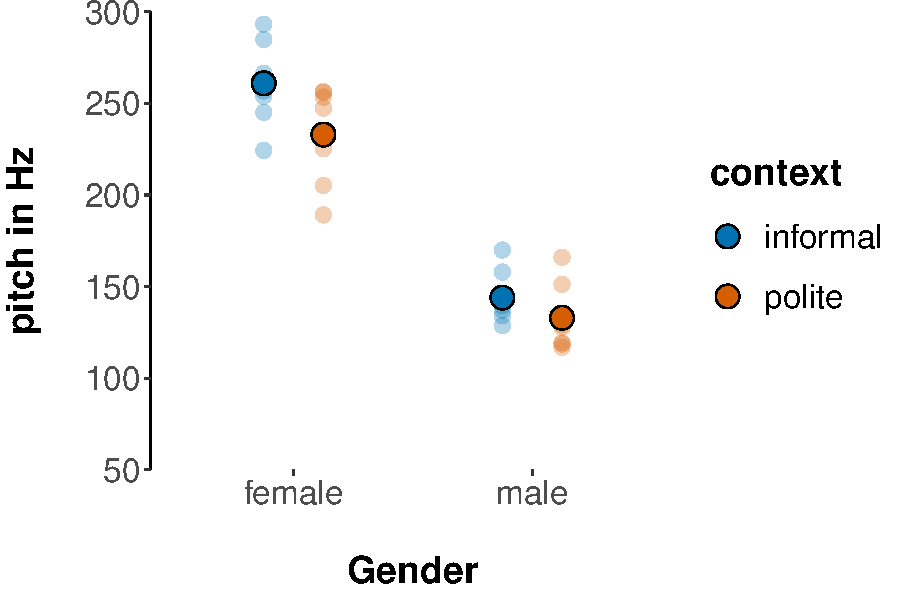
\includegraphics[width = \textwidth]{pics/basic_data_plot.pdf}
    \caption{Basic plot of the data displaying overall averages (thick points) and averages for individual sentences (smaller semitransparent points).}
     \label{fig:BasicPlotData_data}
\end{figure}


Looking at the plot, we might want to shout: ``Eureka! The data confirm all of our
hypotheses!'' But, of course, we need to be more careful. As Bayesians, we would like to
translate the data into an expression of \textbf{evidence}: does the data provide evidence for
our research hypotheses? Or are the observable differences too meager? -- Also, notice that
there is quite a lot of variability between different sentences (the semi-transparent points in Figure 1).
For example, some values from the informal condition for female speakers (orange points in left
column), are lower than their corresponding polite counterparts. Similarly, there could be differences between individual speakers. What we want are precise
estimates of potential differences between conditions. We also want a measure of how confident we can be in these estimates.

\begin{figure}[h]
  \centering
    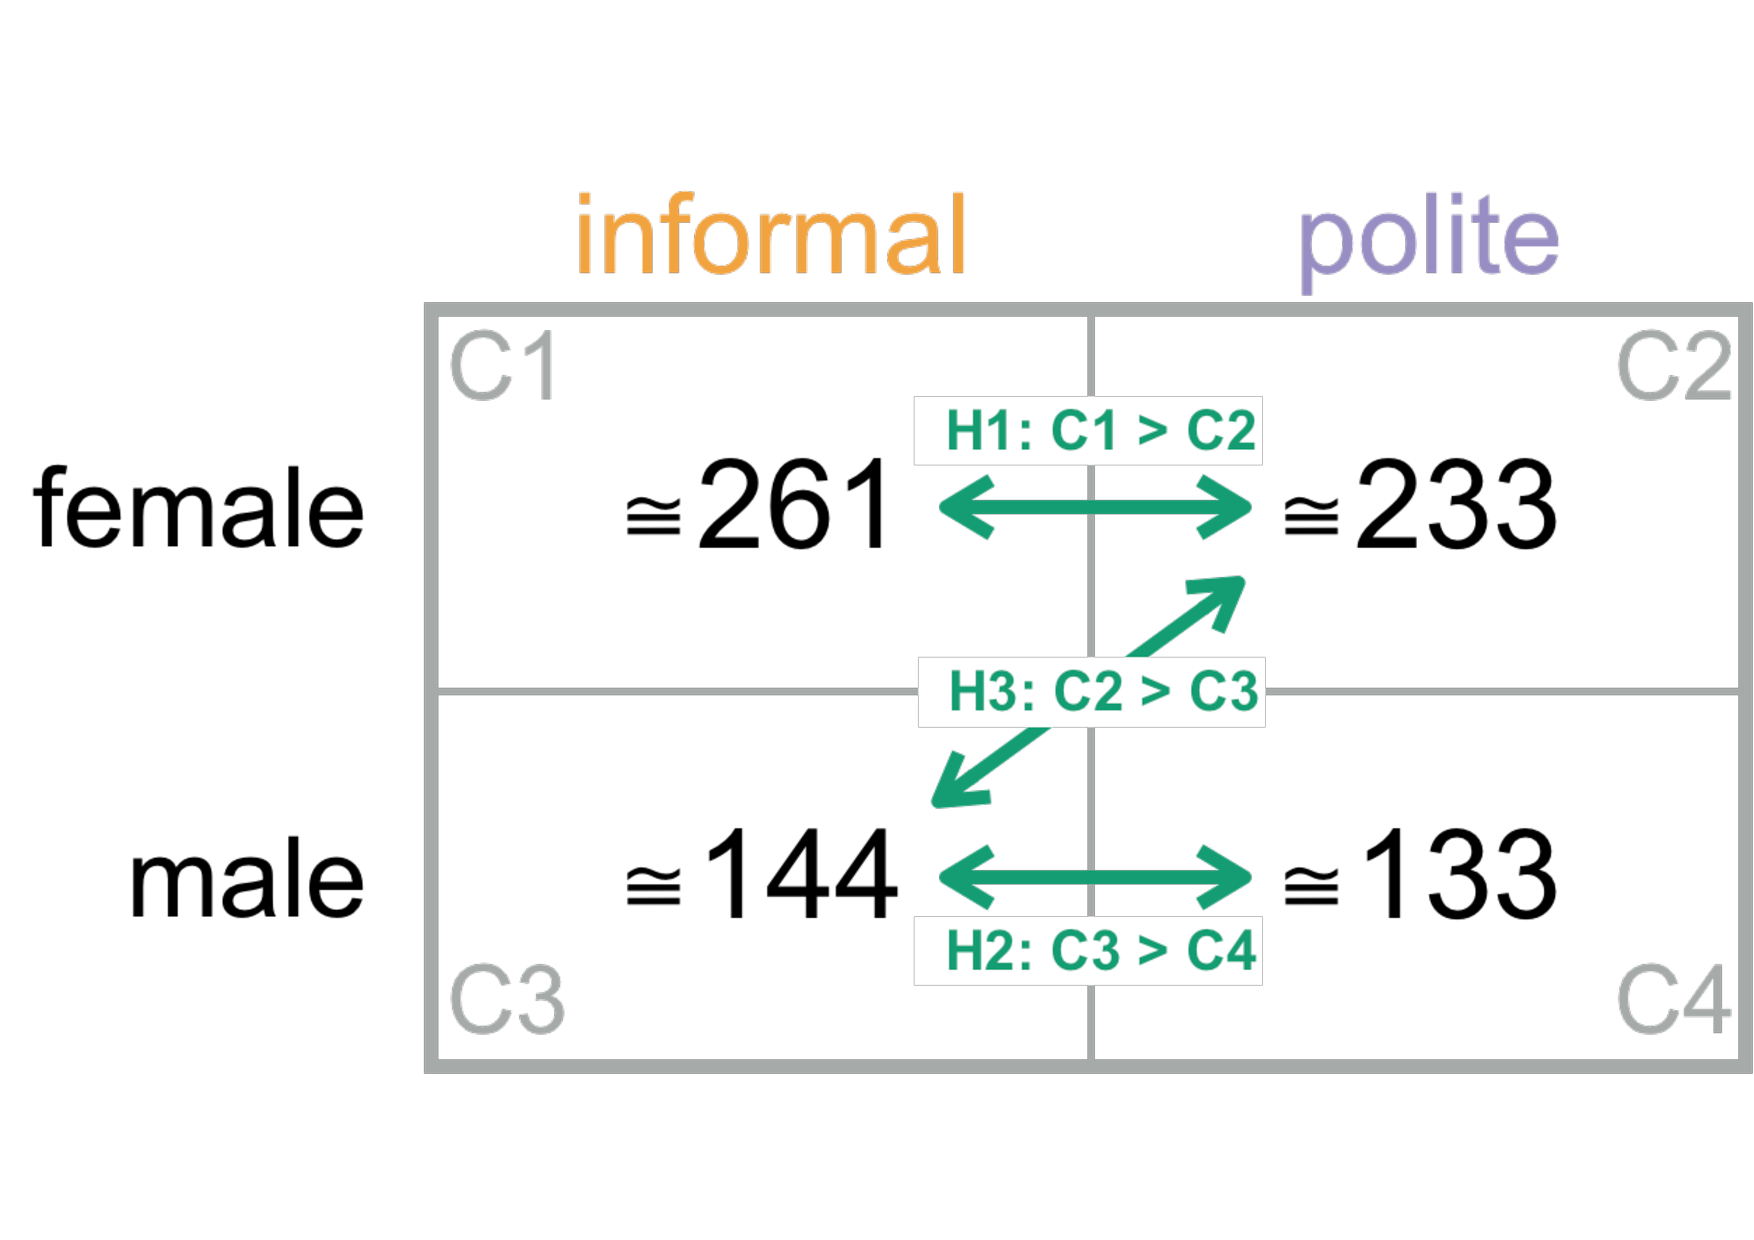
\includegraphics[width = 0.8\textwidth]{pics/table_mean_hypotheses.pdf}
    \caption{Means of each design cell, together with research hypotheses as statements about ordinal relations between cell means.}
    \label{fig:BasicPlotData_table}
\end{figure}

\section{A regression model for our data}

Another way of looking at the data in connection with our research hypotheses is displayed in
Figure~\ref{fig:BasicPlotData_table}. Each cell in this \textbf{design matrix} represents one
unique combination of the gender and the context factor, and the table shows the mean of
observed pitch values for each cell.
%
% \marginnote{In technical terms, this table is the \textbf{design matrix} of our experiment. We
%   have two factors of interest \texttt{context} and \texttt{gender}, each with two levels. The
%   table shows each combination of levels of all relevant factors. The cells in this table are
%   therefore also called \textbf{design cells} \tr{is this marginnote essential or can we maybe
%     get rid of it?}.}
%
Our hypotheses can be related to the comparison between some of these cell-based means.
H1 makes a statement about the comparison between C(ells) 1 and 2 (the context effect for female speakers); H2 makes a statement about C3 and C4 (the context effect for male speakers); and H3 makes a statement about C2 and C3 (the difference between informal male speakers and polite female speakers).

One way of testing our hypotheses using a Bayesian approach to data analysis, is to ask whether the relevant differences between cell means are \textit{credibly different from zero}. This is jargon for asking whether, given the observed data, we should believe that the relevant cell means are different from each other. The fact that we are now in Bayesian land should hit us when we hear the phrases ``credibly different'' and e`should believe''. Bayesian thinking is about updating beliefs based on observations. And we express our beliefs as as probability distributions. 
At first, this may appear scary or technically involved. But at the end of the day, the intuitions captured by this approach are arguably very natural, and perhaps even easier to understand than the reasoning underlying other approaches to statistical inference. Let's walk through our Bayesian approach step-by-step.

First, let's look at the \textbf{regression model} we want to use.
Our regression model assumes that pitch values observed in each cell are
sampled from a population that is normally distribution, where each cell $c_i$ has its own mean $\mu_i$. We are interested in the probability of one cell mean being larger than another cell mean, i.e., the probability that $\mu_i > \mu_j$. Put differently, we are interested in the probability that the difference between $\mu_i$ and $\mu_j$ is larger than zero: $\mu_i - \mu_j > 0$.
%and since, let's say, it is easier to test whether a value is bigger than zero, we can encode the cell means like in Figure~\ref{fig:coefficients_table}. \tr{I cannot see this in the figure. The figure merely displays how we calculate the individual cell mean in a regression}
Figure~\ref{fig:coefficients_table} illustrates the encoding scheme of our cell means in terms of a regression analysis. It assumes that
there is a \textbf{reference level} for each factor. Here it is the level \texttt{female} for
the factor \texttt{gender} and the level \texttt{informal} for the factor
\texttt{context}.\marginnote{This is so-called \textbf{dummy coding} of the regression
coefficients. Other coding schemes exist, but are not discussed here.} 
  
All cell means can then be expressed in terms of differences between the \textbf{intercept}
$\beta_0$ which is the cell mean of the reference level (here, the cell mean of female subjects
in informal contexts), deviations from this \textbf{reference cell} for each individual factor
($\beta_{\text{male}}$, and $\beta_{\text{polite}}$), and a so-called \textbf{interaction term}
$\beta_{\text{pol\&male}}$. In other words, our regression estimates the mean of the reference
level and estimates how much we need to adjust this mean when we change either the context
level (C2), the gender level (C3), or both (C4). The $\beta$ terms are also called
\textbf{coefficients}. They are \textbf{free parameters} of the model.

\begin{figure}[]
  \centering
    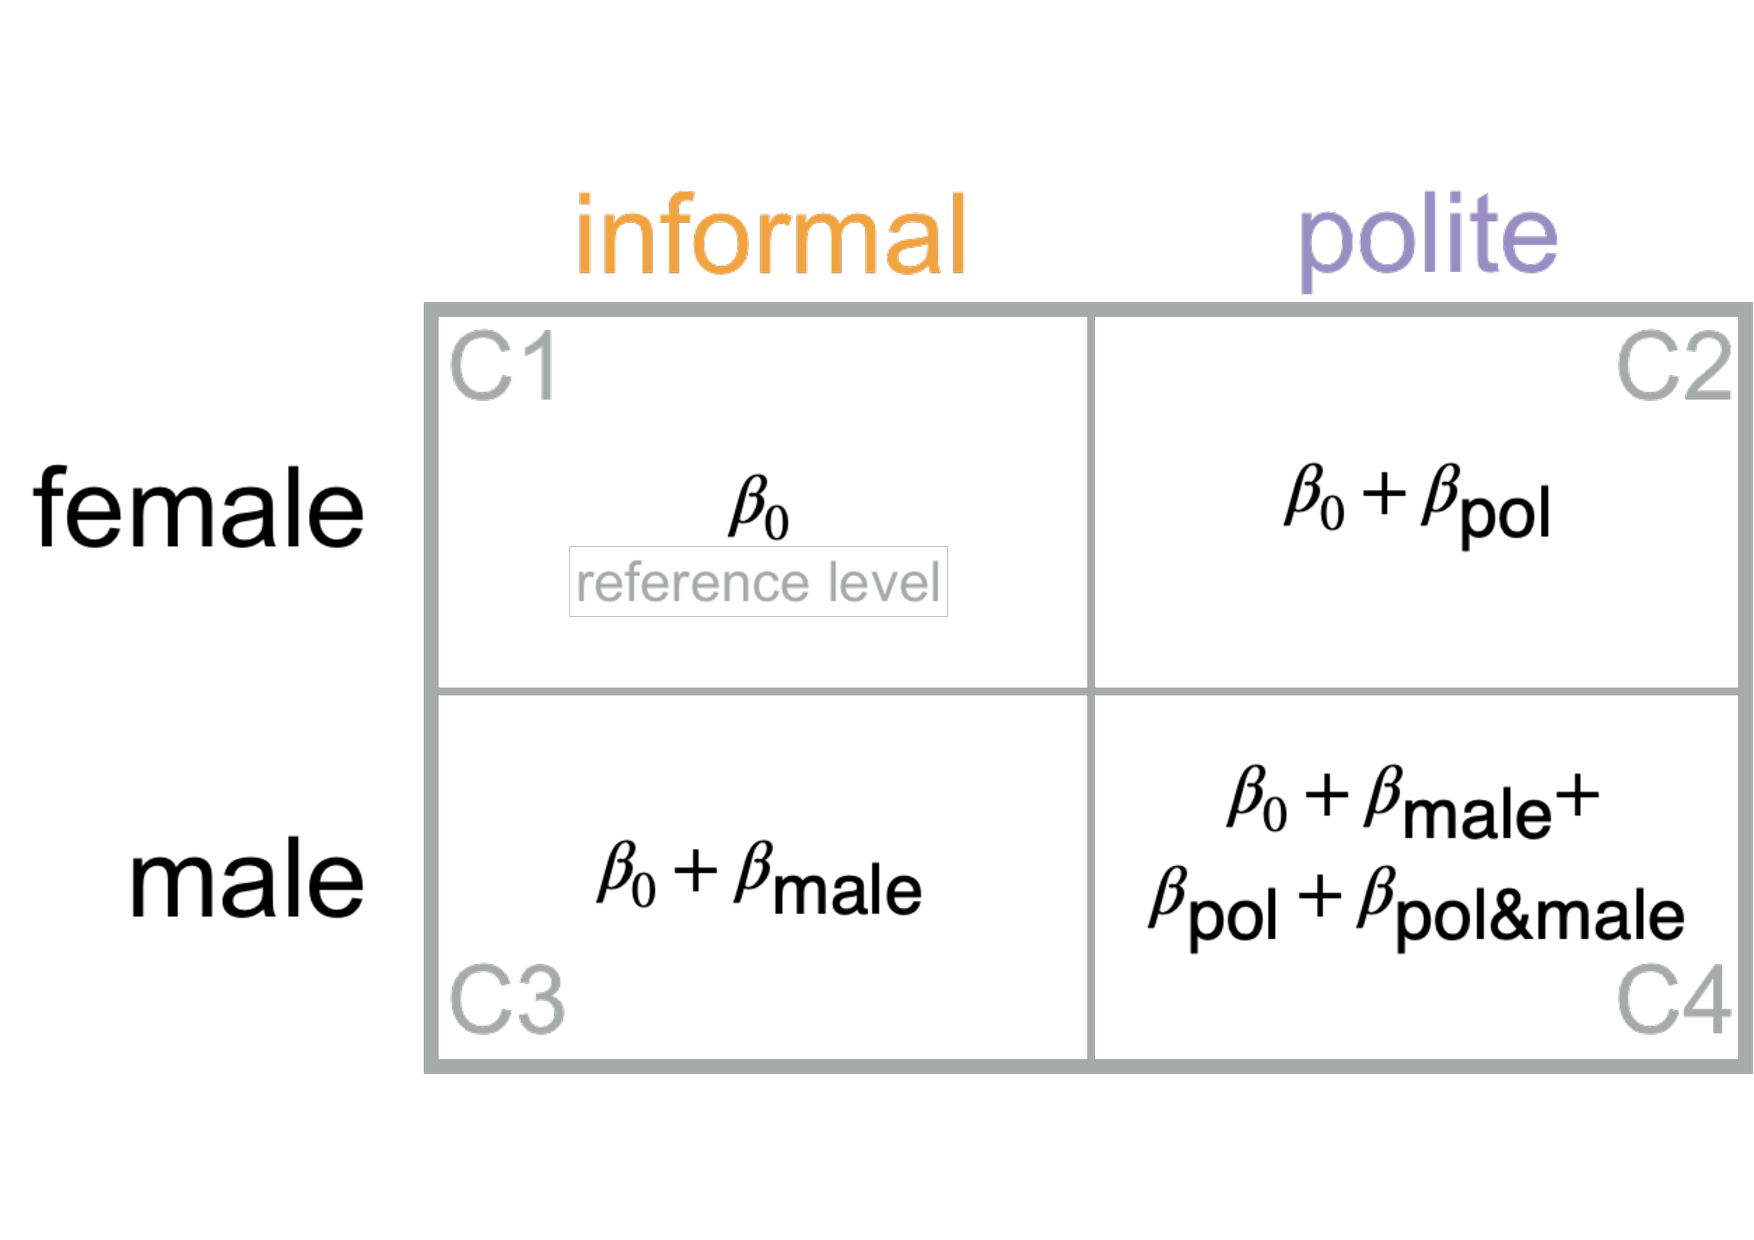
\includegraphics[width = 0.8\textwidth]{pics/table_coefficients.pdf}
    \caption{Coefficients of a dummy-coded regression model for the factorial $2 \times 2$ design.}
    \label{fig:coefficients_table}
\end{figure}

\begin{InfoBox}[]
\centering
\colorbox{mygray}{\centering
  \begin{minipage}{1.0\textwidth}

    \emph{Bayesian inference: priors, likelihoods and posteriors}
    \medskip

    Jones is a rational scientist. She has recently inherited her grandma's lucky coin. Jones suspects that grandma's coin might be a trick coin, but she is not
    sure. She is determined to find out. How? Well, naturally, by rationally updating her
    \emph{prior beliefs} about the coin's bias to obtain a new \emph{posterior belief} based on
    empirical observation (outcomes of coin flips). Central to this updating is Jones'
    \emph{likelihood function}, which encodes how likely each relevant coin bias may have
    generated the observed data.
    
    \paragraph{Prior beliefs.} Jones knows that there are two coin factories: one produces fair
    coins, the other produces coins which give heads three times more often than tails. She
    believes that it's equally likely that the coin is from either factory. In formal notation,
    if $\theta$ is the coin's bias, i.e., the probability with which it lands heads when
    tossed, Jones' \emph{prior beliefs} are:
    \begin{align*}
      P(\theta = \nicefrac{1}{2}) = P(\theta = \nicefrac{3}{4}) = \nicefrac{1}{2}
    \end{align*}


    \paragraph{Likelihood.} The bias $\theta$ is, by definition, the probability of the coin
    landing heads on the next trial. Let's assume that Jones tosses the coin only once (hm,
    maybe not so rational a scientist after all? or just too busy?). If $D\!=\!\set{\text{heads}, \text{tails}}$ is the set of potential outcomes of this experiment, the \emph{likelihood
      function} determines the likelihood of observing each observation {$d\!\in D$} for each
    $\theta$, which in our case is:
    \begin{align*}
      P(D = \text{heads} \mid \theta) & =  \theta \\
      P(D = \text{tails} \mid \theta) & = 1 - \theta
    \end{align*}

    \paragraph{Posterior beliefs.} Jones observes that the coin landed heads. What should she
    believe now? By \emph{Bayes rule} her posterior beliefs are defined as:
    \begin{align*}
      P(\theta \mid D = \text{heads}) = \frac{P(\theta) P(D = \text{heads} \mid \theta)}{\sum_{\theta'}P(\theta') P(D = \text{heads} \mid \theta')}
    \end{align*}
    Jones' posterior belief that the coin is biased to land heads three times more likely than tails is therefore:
    \begin{align*}
      & P(\theta = \nicefrac{3}{4} \mid D = \text{heads}) =  \\
      & \frac{P(\theta = \nicefrac{3}{4}) \ P(D = \text{heads} \mid \theta = \nicefrac{3}{4})}{P(\theta = \nicefrac{3}{4}) \ P(D = \text{heads} \mid \theta = \nicefrac{3}{4}) + P(\theta = \nicefrac{1}{2}) \ P(D = \text{heads} \mid \theta = \nicefrac{1}{2})} = \\
      & \frac{\nicefrac{1}{2} \ \nicefrac{3}{4}}{\nicefrac{1}{2} \ \nicefrac{3}{4} + \nicefrac{1}{2} \ \nicefrac{1}{2}} = \frac{\nicefrac{3}{8}}{\nicefrac{7}{8}} = \frac{3}{5} 
    \end{align*}
    After making her observation, rational Jones has updated her initial level of credence of $0.5$ in the assumption that the coin is biased to $0.6$.
    
  \end{minipage} \par
  } \par
  \begin{center}
    Info Box 1: Priors, likelihood and posteriors in Bayesian inference.
  \end{center}
  % \caption{\label{InfoBox:asymptotic_CIs} Here is my caption}  
\end{InfoBox}


\section{A Bayesian analysis of a (fixed effects) regression model}

Having spelled out a model like the above, a Bayesian analysis asks: What are credible values for the model's parameters, i.e., what should a rational reasoner believe about the values of,
in particular, the coefficients $\beta_0$, $\beta_{\text{pol}}$, $\beta_{\text{male}}$ and $\beta_{\text{pol\&male}}$ given the reasoner's initial beliefs and the data, on the assumption that the model is true?
%
\marginnote{Info Box~1 provides some background on Bayesian reasoning}
%
Formally, if $\theta$ is a vector of parameter values of the model, we are interested in the \textbf{posterior distribution} $P(\theta \mid D)$, which assigns a non-negative number to each tuple of parameters in proportion to how likely that tuple is.
From a Bayesian point of view, the model consists of a \textbf{likelihood function} $P(D \mid \theta)$, which specifies how likely an observation of data $D$ is for each value of parameters $\theta$, and a \textbf{prior distribution} $P(\theta)$, which specifies how likely we (the rational reasoners) believe each tuple of parameter values is in the first place.
%
\marginnote{Supplying a \textbf{prior}, really just \textit{any} prior, is important to get a
  Bayesian analysis off the ground; a circumstance which is discussed controversially. For many
  practical purposes, however, the precise choice of prior is not decisive and tools like the
  \texttt{brms} package which we will use here will default to generically reasonable choices
  of priors for your model (more on this below).}
%
With these ingredients, we can compute the posterior distribution by Bayes rule, as follows:
\begin{eqnarray*}
  P(\theta \mid D) = \frac{P(\theta) \ P(D \mid \theta)}{ \int P(\theta') \ P(D \mid
  \theta') \textrm{d}\theta'}
\end{eqnarray*}

The R package \texttt{brms} \citep{buerkner2016brms} makes it easy to run Bayesian regression models. It uses a very similar formula syntax as related packages for regression analysis. In our case, we want to regress the dependent variable \texttt{pitch} against the independent variables \texttt{gender} and \texttt{context} and their two-way interaction. This model is expressed by the formula:

\bigskip

\begin{minipage}[]{\textwidth}
\begin{lstlisting}[language=R]
# formula for (fixed effects) regression model
formulaFE = pitch ~ gender * context
\end{lstlisting}
\end{minipage}

The Bayesian model can then be fitted with the function \texttt{brm} from the \texttt{brms} package. We only need to specify the formula and supply the data:

\bigskip

\begin{minipage}[]{\textwidth}
\begin{lstlisting}[language=R]
# run regression model in brms
modelFE = brm(
  formula = formulaFE,
  data = politedata)
\end{lstlisting}
\end{minipage}

\noindent The \texttt{brms} packages uses the probabilistic programming language \texttt{Stan}
in the background. \texttt{brms} basically translates our syntax into Stan code and
executes it. The Stan code  is then translated to C++ (hence the message about ``compiling
C++'' when you run this code). Conceptually, Stan obtains samples from the posterior
distribution, based on an algorithm called \emph{Hamiltonian Monte Carlo}. This is an instance
of a more general class of algorithms, called \emph{Markov Chain Monte Carlo} methods. The
purpose of these methods is to return representative samples from the posterior distribution.
If you are interested in finding out more about this 'sampling stuff', check out Info Box~2?

\begin{InfoBox}[]
\centering
\colorbox{mygray}{\centering
  \begin{minipage}{1\textwidth}

    \emph{Markov Chain Monte Carlo (MCMC) sampling}
    \medskip
 
    Bayesian ideas are old, but they have seen a revival recently, in large part due to
    advances in computer science (notably: clever algorithms, not just faster computers). To
    understand this, consider Bayes rule for data analysis. We have a prior $P(\theta)$ over
    parameter vector $\theta$ and a likelihood function $P(D\mid\theta)$. We want to compute
    the posterior distribution
    :
    \begin{eqnarray*}
      P(\theta \mid D) = \frac{P(\theta) \ P(D \mid \theta)}{ \int P(\theta') \ P(D \mid
      \theta') \textrm{d}\theta'}
    \end{eqnarray*}
    If $\theta$ is a large vector of parameters (e.g., in a hierarchical regression model), it
    might be quite impossible to compute the integral in the denominator. Fortunately, clever
    algorithms like MCMC allow us to draw \textbf{representative samples} from the
    posterior distribution without having to calculate the integral-of-doom.

    \medskip
    
    For common applications, it is not required to understand MCMC
    algorithms in full detail. It suffices to know that samples are collected by starting at
    (usually random) initial parameter values, and then ``jump around parameter space'' in such
    a way that, in the limit, they will visit any particular tuple of parameter values with
    exactly its posterior probability. So, these algorithms are guaranteed to give us
    representative samples, given unlimited time to jump around. To make sure the samples we
    have are still good enough, we take some precautions and use some diagnostic tools for
    quality control.

    \medskip
    
    To ensure trustworthiness of samples, we routinely run several \textbf{chains}, i.e., we
    start the ``jumping around'' at different random initial starting points and check whether
    the different chains reached a similar outcome. We do this by plotting (so-called
    \emph{trace plots}) and the \textbf{$\hat{R}$-value} which is included in the \texttt{brm}
    model summary. An $\hat{R}$-statistic compares the variance of the samples within each
    chain to that from all samples across chains (similar to ANOVA). If the $\hat{R}$-value is
    below 1.1, we commonly assume that the chains have converged sufficiently.

    \medskip
  
    In practice, the \textrm{brm} model summary and the messages during the fitting process will inform you about potential problems with convergence, and will frequently offer good advice for how to solve the issue. One quick and simple solution is increasing the number of samples (specifying the option \texttt{iter} in the \texttt{brm} function call).
   
  \end{minipage} \par
  } \par
  \begin{center}
    Info Box 2: Background on sampling methods \& diagnostics.
  \end{center}
\end{InfoBox}


You can type in \texttt{modelFE} in order to get a summary of the model fit. It should look like the following output.

\bigskip

\begin{minipage}[]{1.2\textwidth}
\begin{rc}
> modelFE
 Family: gaussian 
  Links: mu = identity; sigma = identity 
Formula: pitch ~ gender * context 
   Data: politedata (Number of observations: 83) 
Samples: 4 chains, each with iter = 2000; warmup = 1000; thin = 1;
         total post-warmup samples = 4000

Population-Level Effects: 
                   Estimate Est.Error l-95% CI u-95% CI Eff.Sample Rhat
Intercept            260.68      8.07   244.99   276.78       2409 1.00
genderM             -116.09     11.44  -138.37   -93.80       2094 1.00
contextpol           -27.38     11.33   -50.01    -5.98       2092 1.00
genderM:contextpol    15.74     16.38   -17.03    49.13       1831 1.00

Family Specific Parameters: 
      Estimate Est.Error l-95% CI u-95% CI Eff.Sample Rhat
sigma    36.15      2.87    30.93    42.40       3652 1.00

Samples were drawn using sampling(NUTS). For each parameter, Eff.Sample 
is a crude measure of effective sample size, and Rhat is the potential 
scale reduction factor on split chains (at convergence, Rhat = 1).
\end{rc}
\end{minipage}

Lines 2--5 give us information about the model and the data used. Lines 6 and 7 tell us about
the sampling procedure (see Info Box~2 for more information). Lines 9--14 contain information about our
parameters of interest. We will discuss them in detail below. Lines 16--18 contain information
that look similar to those in lines 9--14. This is the estimation of the standard deviation
\texttt{sigma}, describing the variance of the assumed normal distributions (which describe the
distribution of measures in each design cell). Finally, lines 20--22 contain general
information about the model fit and the information presented in this summary.\marginnote{If
  the model failed to converge or other problems occurred, you would see an informative message
  in the last part of this summary (see Info Box~3).}

Let us look at lines 9--14 in detail now. What these lines give us is a table with four rows, each of which corresponds to a parameter in the model, namely the coefficients shown in Figure~\ref{fig:coefficients_table}. The variable \texttt{Intercept} refers to our $\beta_0$, which represents the mean of our reference level in cell 1 (female speakers in polite contexts). The variable \texttt{genderM} corresponds to our $\beta_{\text{male}}$, \texttt{contextpol} corresponds to our $\beta_{\text{pol}}$, and \texttt{genderM:contextpol} is the interaction term $\beta_{\text{pol\&male}}$. For each of these parameters, the table contains very useful summary statistics based on the samples returned from the model fit.
%
\marginnote[-2.5cm]{Intuitively, the 95\% credible interval is the range of values that we can often practically consider credible enough to care about.}
%
More details about the information given in the other columns can be found in Info Box~3.

\begin{InfoBox}[t]
\centering
\colorbox{mygray}{\centering
  \begin{minipage}{1.0\textwidth}

    \emph{Information displayed in the summary of a \texttt{brm} model fit}
    \medskip

    Lines 6--7 of the summary of \texttt{modelFE} tell us that we collected a total of 4000 samples from the posterior distribution. These came from four chains, each running for 2000 iterations, but discarding the first 1000 samples as \textbf{warm up}, since the initial starting point might be quite ``unrepresentative'' (see also Info Box~2).
    
    From the table in lines 9--14, the column \emph{Estimate} gives the mean of the obtained
    samples, thereby approximating the mean of the posterior distribution (beliefs we should
    hold) about each parameter. For example, the parameter \texttt{Intercept} is estimated to
    have a mean of about $261$, which (here) coincides with the mean of the data points in cell
    1, as shown in Figure~\ref{fig:BasicPlotData_table}. \emph{Est.Error} is the estimation
    error, an indication of the certainty we should have about the whole inference procedure.
    The columns \texttt{l-95\% CI} and \texttt{u-95\% CI} give the lower and upper bound of the
    95\% credible interval for each parameter, as discussed in the main text. The column
    \texttt{Eff.Sample}, for efficient samples, gives a rough measure of how many of all the
    samples we took (4000 in our case) are contributing non-redundant information to our
    estimation. The higher this number, the better. Finally, we get the \texttt{Rhat} column with the $\hat{R}$-values for each parameter (see Info Box~2).
    
  \end{minipage} \par
  } \par
  \begin{center}
    Info Box 3: Information in summaries of \texttt{brm} model fits.
  \end{center}
\end{InfoBox}


For our current purposes, the information in  columns \texttt{l-95\% CI} and \texttt{u-95\% CI} is most important.
These numbers give the lower and upper bounds of a \textbf{95\% credible interval}.
Take the parameter \texttt{contextpol}, corresponding to our coefficient $\beta_{\text{pol}}$.
This parameter corresponds to the estimated adjustment of the mean of the reference level when we change the context level to polite.
The 95\% CI is roughly [-50;-6].
We could take values outside of this interval to be sufficiently unlikely to be ignorable for most purposes.
Consequently, a very special value for this parameter has to be considered implausible, namely 0.
In other words, this analysis suggests that 0 is a very unlikely value for the coefficient $\beta_{\text{pol}}$; rather we should believe that $\beta_{\text{pol}}$ is most likely negative. --- Hurray!
This directly addresses our first research hypothesis.
In a research paper we could now write: ``Based on the regression model, the data suggests that H1 is likely true.''

How likely is it that $\beta_{\text{pol}}$ is smaller than 0? ---Instead of simply making a binary thumbs-up / thumbs-down decision, it would be even more elegant, if we could put a number to it. As Bayesians, we fortunately can. To see how this works, let us have a more intimate look at the samples that the \texttt{brm} function returns. We can access the samples of a model fitted with \texttt{brm} with the function \texttt{posterior\_samples}:

\bigskip

\begin{minipage}[]{\textwidth}
\begin{lstlisting}[language=R]
# extract posterior samples 
post_samples_FE = posterior_samples(modelFE)
head(post_samples_FE)
\end{lstlisting}
\end{minipage}

The output of this could look like this:

\bigskip

\begin{minipage}[]{1.2\textwidth}
\begin{rc}
> head(post_samples_FE)
  b_Intercept b_genderM b_contextpol b_genderM:contextpol sigma   lp__
1       270.6    -123.5        -22.1                 16.1  36.0 -422.4
2       268.7    -131.0        -36.8                 36.1  39.6 -421.1
3       255.8    -108.9        -20.2                 11.7  39.2 -420.5
4       259.4    -115.7        -29.4                 12.8  31.2 -420.8
5       256.5    -106.0        -15.2                -11.7  36.2 -420.8
6       245.8    -112.2         -9.6                 17.6  39.5 -423.1
\end{rc}
\end{minipage}

What you see here is the top 6 rows of a data frame with columns for each parameter and 4000 rows, corresponding to each sample of that parameter (so our sampling method has generated 4000 values for each parameter, where each row is a sample from the posterior distribution $P(\theta \mid D)$).
%
\marginnote{The column \texttt{lp\_\_} contains the log-probability of the data for the parameterization in each row. This is useful for model comparison and model criticism but not important for our current adventures.}
%
We can use these samples to produce density plots reflecting out posterior distribution. The plot in Figure~\ref{fig:Posteriors_FE}
shows, for each of the four main model parameters an estimate of the posterior density. Each
curve shows how much credence we should put on particular parameter values. For example, we see
that our beliefs concerning plausible values for the mean of cell 1 (female speakers in polite
contexts, the reference cell) should hover around 261, roughly spreading from about 240 to 280. We also see that all values that receive substantial probability density for \texttt{context:pol} (our $\beta_{\text{pol}}$) are negative (as captured in the 95\% CI discussed above). Zero is estimated to be a comparatively unlikely value for this parameter.

\begin{figure}
  \centering
  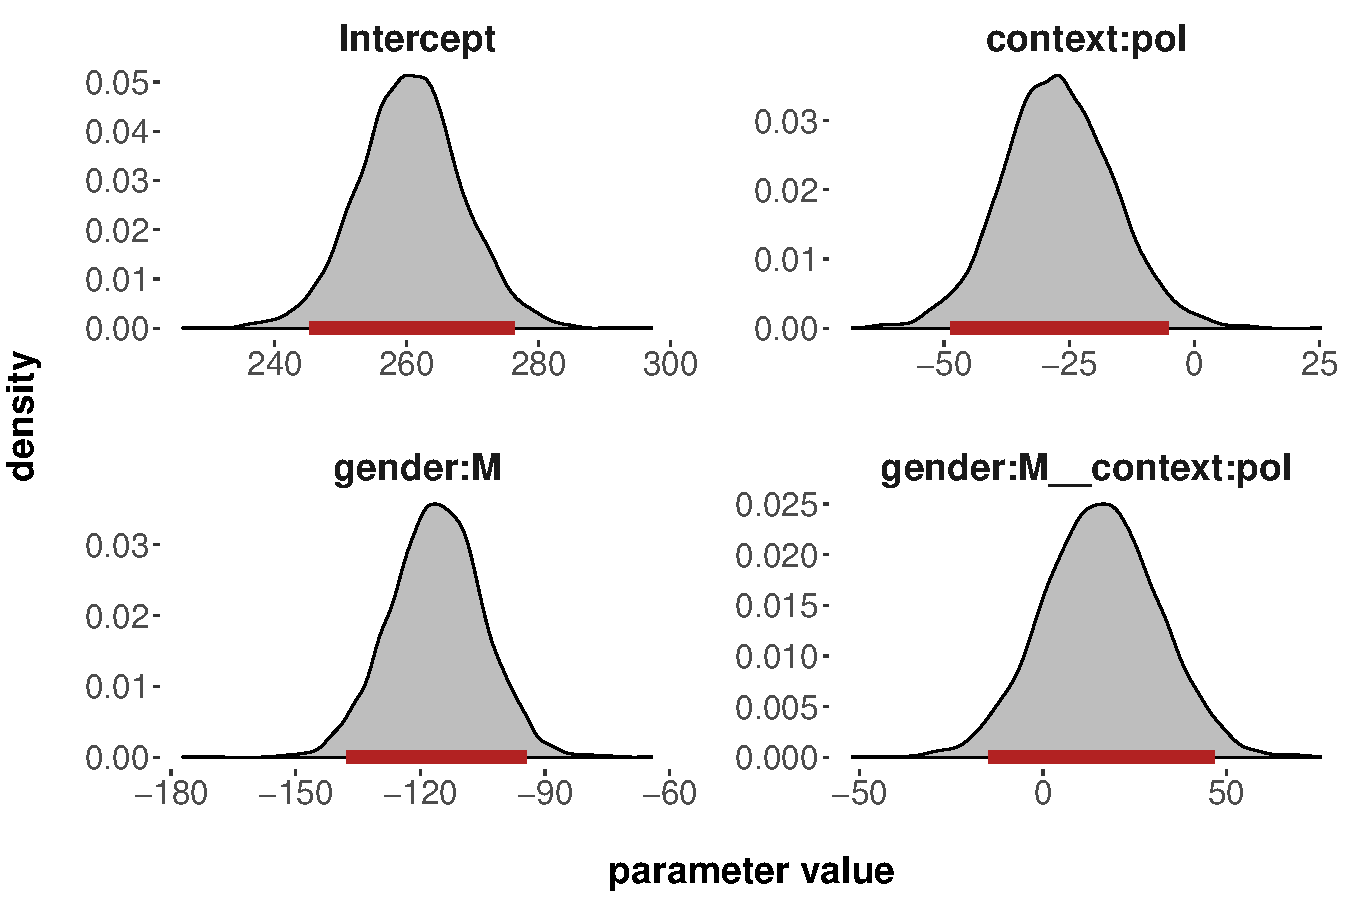
\includegraphics[width=\textwidth]{pics/posterior_density_FE.pdf}
  \caption[Posterior over coefficients in fixed-effects model]{Posterior density of parameter
    values in the fixed-effects regression model. The thick red lines indicate the 95\%
    credible intervals, i.e., the range of parameter values that it is reasonable to believe
    in.}
  \label{fig:Posteriors_FE}
\end{figure}

Now, here comes a nice gadget. Based on the samples obtained for \texttt{contextpol} ($\beta_{\text{pol}}$), it is very easy to estimate our belief that $\beta_{\text{pol}}$ is indeed negative. We simply have to calculate the proportion of samples that were negative. That's all. For instance, with the code below, which reveals that given the data and the model, the posterior probability of the proposition that $\beta_{\text{pol}} < 0$ is about 0.99275. This is very close to 1!  

\bigskip

\begin{minipage}[]{\textwidth}
\begin{lstlisting}[language=R]
# proportion of negative samples for parameter b_contextpol
# this number approximates P(b_contextpol < 0 | model, data)
mean(post_samples_FE$b_contextpol < 0)
\end{lstlisting}
\end{minipage}

As an interim summary, we have seen how to run a Bayesian regression analysis with the \texttt{brms} package and deal with its output. We have also seen that the output can be interpreted in very intuitive ways (e.g., ``The probability of H1, given our model, priors, and data, is more than .99'').

Unfortunately, what we have not seen yet is what our model and data say about hypotheses 2 or 3. This is because there is no single parameter in the (dummy-coded) regression model that corresponds to the differences between cells 3 and 4 (for hypothesis 2) and cells 2 and 3 (for hypothesis 3). Notice that this problem is not specific to Bayesian analyses, but inherent in the way the regression coefficients were set up.
%
\marginnote{A potential way of testing different hypotheses of the kind we have set our here, is to run different regression analyses, each with a different reference cell. This is a rather unhandy work flow. It wouldn't help with hypothesis 3 either, which compares the cell means in our design matrix``diagonally'': there is no way of changing the reference level of either factor such that dummy coding gives us a single coefficient as the difference between cells 2 and 3.}
%
Fortunately, we can recover information about any derived measure from the obtained samples. Here's how:

Take hypothesis 3 which requires us to compare cells 2 and 3. The hypothesis states that
$\beta_0 + \beta_{\text{pol}} > \beta_0 + \beta_{\text{male}}$, which reduces to
$\beta_{\text{pol}} > \beta_{\text{male}}$. We can approximate the posterior probability that
this is true based on the samples that we obtained for our model in the same general way as
before, namely:

\bigskip

\begin{minipage}[]{1.1\textwidth}
\begin{lstlisting}[language=R]
# proportion of samples where the mean for cell 2 was larger 
# than that of cell 3 
# this number approximates the quantity:
#    P(b_contextpol > b_genderM | model, data)
mean(post_samples_FE$b_contextpol > post_samples_FE$b_genderM)
\end{lstlisting}
\end{minipage}

Based on the posterior samples we obtained, the estimated probability is 1. That's a strong result. If the model was true, then, given the data, our certainty that hypothesis 3 is true should be pretty much almost at ceiling.

To conclude this section, the Bayesian approach to regression modeling allows us to retrieve all direct comparisons between cells in a factorial design (all possible comparisons). It also allows us to retrieve quantitative information about our hypotheses in a way which is easy to communicate and understand. We can calculate the (estimated) posterior probability that a particular hypothesis holds. 

\subsection{The \texttt{faintr} package}

To make the comparison of pairs of cells even easier and applicable for even bigger factorial designs, this tutorial comes with a little R package, the \texttt{faintr} package.
%
% \marginnote[-1.5cm]{The name \texttt{faintr} is indicative of the possibility that the package might break down unexpectedly (we might consider renaming after more extensive testing), but also alludes to ``\emph{fa}ctorial design'' and ``\emph{int}erpretation'' somehow.}
%
You can install the package from GitHub with the \texttt{devtools} package, as follows:

\medskip 

\begin{minipage}[]{1.3\textwidth}
\begin{lstlisting}[language=R]
# load package to allow installation from GitHub
library(devtools)
# install package with convenience function for Bayesian regression 
# models for factorial designs from GitHub
install_github(
  repo = 'michael-franke/bayes_mixed_regression_tutorial', 
  subdir = 'faintr',
  build_vignettes = TRUE)
# load the just installed package
library(faintr)
\end{lstlisting}
\end{minipage}

The \texttt{faintr} package provides two main helper functions.
%
\marginnote{You can read a vignette with more information on the \texttt{faintr} package if you type \texttt{vignette("faintr\_basics")} after installing the package.}
%
The function \texttt{extract\_posterior\_cell\_means()}
takes as input the fitted regression model and outputs samples for all design cell means, and a comparison of all design
cells against each other. For example, although the model fitted $\beta$-coefficients, we can reconstruct posterior estimates of each cell's means by typing:

\begin{minipage}[]{1.3\textwidth}
\begin{lstlisting}[language=R]
extract_posterior_cell_means(modelFE)$predictor_values
\end{lstlisting}
\end{minipage}

\vspace*{-0.5cm}

\noindent Using these reconstructed samples, we can plot approximate posterior estimates for each cell, as in Figure~\ref{fig:Posteriors_cell_means}

\begin{figure}
  \centering
  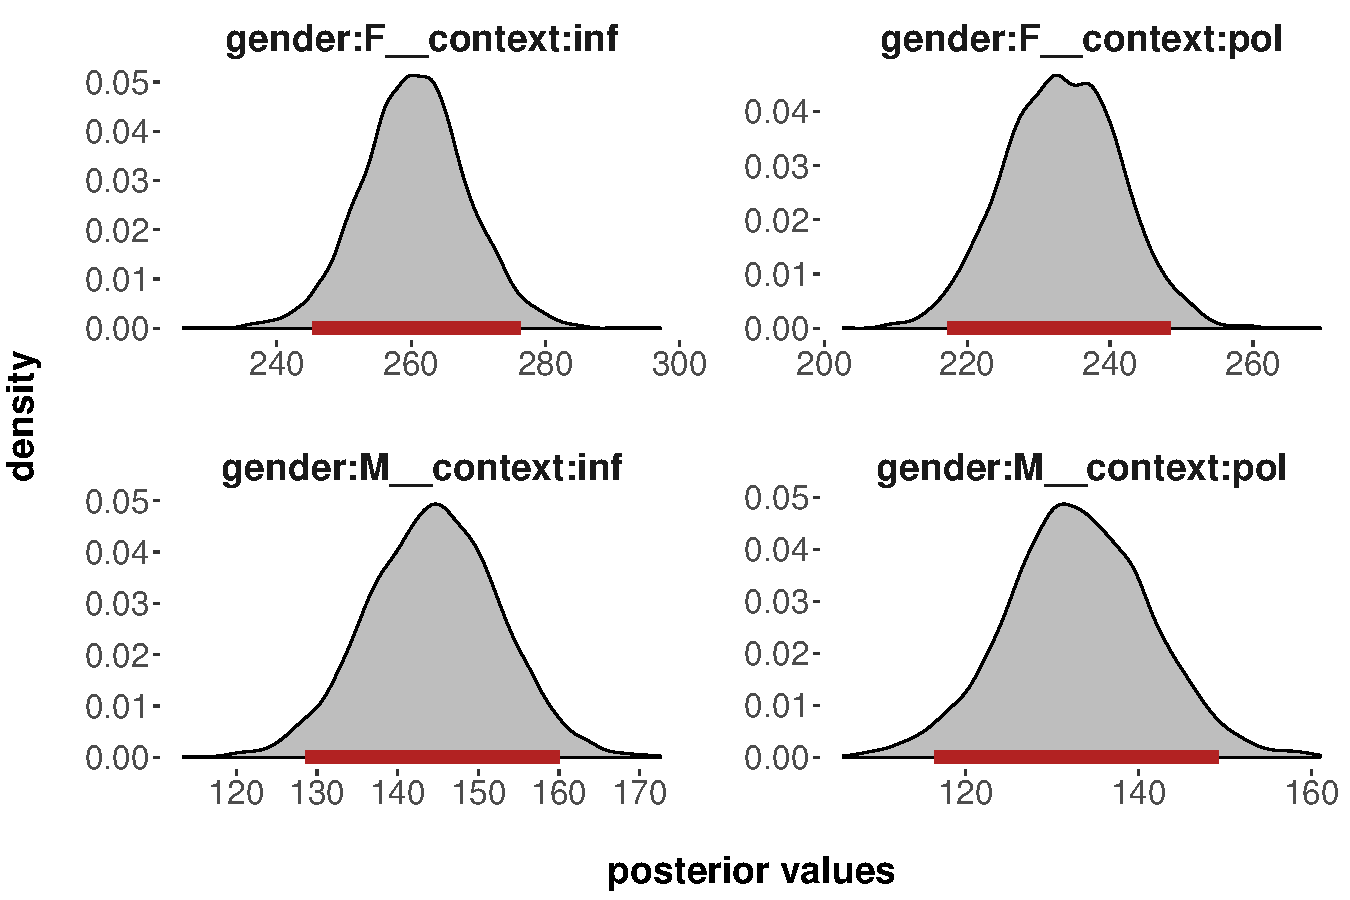
\includegraphics[width=\textwidth]{pics/posterior_density_cell_means.pdf}
  \caption[Posteriors over cell means in fixed-effects model]{Posterior density of cell means
    in the fixed-effects regression model. The thick red lines indicate the 95\% credible
    intervals, i.e., the range of parameter values that it is reasonable to believe in.}
  \label{fig:Posteriors_cell_means}
\end{figure}


Another helpful function is \texttt{compare\_groups()}, which takes as input a fitted
regression model together with a specification of which two (subsets of) cells to compare
against each other. For example, we can compare (diagonally) the cells for female speakers in
polite contexts with male speakers in informal contexts with this call:

\begin{minipage}[]{1.3\textwidth}
\begin{lstlisting}[language=R]
compare_groups(
  model = modelFE, 
  lower = list(gender = "M", context = "inf"),
  higher = list(gender = "F", context = "pol")
)
\end{lstlisting}
\end{minipage}

The output looks like this:

\medskip

\begin{minipage}[]{\textwidth}
\begin{rc}
Outcome of comparing groups:
 * higher:  gender:F context:pol 
 * lower:   gender:M context:inf 
Mean 'higher - lower':  88.97 
95% CI: [ 67.33 ; 110.2 ]
P('higher - lower' > 0):  1 
\end{rc}
\end{minipage}

Using the \texttt{compare\_groups()} function, the source code provides a convenient function to
produce the posterior probability of the three hypothesis relevant for this tutorial:

\medskip

\begin{minipage}[]{\textwidth}
\begin{rc}
> get_posterior_beliefs_about_hypotheses_new(model_MaxRE)
# A tibble: 3 x 2
  hypothesis                      probability
  <chr>                                 <dbl>
1 Female-polite < Female-informal       0.973
2 Male-polite < Male-informal           0.850
3 Male-informal < Female-polite         0.922
\end{rc}
\end{minipage}

\section{Priors}

One important difference between traditional frequentist and Bayesian inference are priors. Priors are pieces of information about our data that we assume before actually looking at them. Specifying priors has several advantages, both technical and conceptual. First, as a technical advantage, we can use \textbf{regularizing priors} to implement soft constraints on what counts as a plausible parameter setting for the model, thereby reducing the computational resources needed to estimate the model parameters.
%
\marginnote[-1.5cm]{Defining regularizing priors is essential for more complex models which have to estimate many parameters. Regularizing priors can help our model to converge more quickly.}
%
As a conceptual advantage, priors can also express our relevant subjective beliefs about the situation or problem at hand. For example, pitch values (and many other things we measure in nature) cannot be smaller than 0. Human pitch values are also limited to a certain range defined by physiological and bio-mechanical constraints on our laryngeal system. In adults, values larger than let's say 1000 Hz are very unlikely. 
 
But wait a minute. Subjective beliefs? This is science. We are supposed to be objective, right? You are right. We should have a heart of stone and be skeptical about possible relationships in the first place.
Practically, this means the following for us. We should not hesitate to make use of the possibility to bring all the potentially relevant background knowledge to bear when analyzing our data. The formalization of background knowledge should, of course, be made transparent and be explicitly justified. But, of course, we should \emph{not} engineer in the conclusions we would like to obtain eventually! If our research hypothesis is that male voice pitch is lower than female voice pitch, we obviously don't want to specify a prior that assumes the hypothesized relationship before having seen the data. Instead, we should feed our model a \textbf{skeptical} prior about the truth of our research hypothesis. A possible skeptical prior could be the assumption that there is likely \textit{no} relationship between speaker gender and voice pitch (i.e. the average difference is 0). Of course, there might be some variability around this average value (nature is messy after all), so we might want to assume that pitch differences between male and female speakers are normally distributed with an average of 0 and a standard deviation of, say, 50 Hz. Importantly, such a skeptical prior is conservative with regard to our research hypothesis. Our point of departure (before we observed new data) is to assume that there is no effect of gender on pitch. The data need to convince us otherwise.

How does that look in practice?

\begin{itemize}
\item show brms defaults for our model
\end{itemize}

Let's define some priors for our hierarchical model from above. We keep it simple and define a regularizing prior for the intercept (i.e. our reference level) that defines a normal distribution in plausible-pitch-value-land (for convenience we simply pick the mean and sd for our data set). We also define a skeptical prior for all our fixed effects in question (class = b) as normal distributions centered around zero (again, our prior assumption is that there is no difference between conditions).  

\marginnote[-1.5cm]{You can specify every single parameter of your model individually. To see all parameters for which you can specify priors, use the \texttt{get\_prior()} function of \texttt{brms}}

\bigskip

\begin{minipage}[]{1\textwidth}
\begin{lstlisting}[language=R]
priorFE <- c(
  # define a regularizing prior for the intercept within 
  # the range of possible pitch values: a normal distribution 
  # with the mean of 194 and a standard deviation of 66
  prior(normal(194, 66 class = Intercept),
  # define a skeptical prior for all relevant fixed effects
  prior(normal(0, 50), class = b)
)
\end{lstlisting}
\end{minipage}

We add this prior to the model as an argument and calculate the probability for our hypotheses again. We can see that our priors did not affect the posteriors very much.

\bigskip

\begin{minipage}[]{1\textwidth}
\begin{lstlisting}[language=R]
modelFE_prior = brm(formula = pitch ~ gender * context,
	# add prior 
	prior = priorFE,
	data = politedata,
	control = list(adapt_delta = 0.99)
	)    
\end{lstlisting}
\end{minipage}

\begin{minipage}[]{\textwidth}
\begin{rc}
> get_posterior_beliefs_about_hypotheses_new(modelFE_prior)
# A tibble: 3 x 2
  hypothesis                      probability
  <chr>                                 <dbl>
1 Female-polite < Female-informal       0.983
2 Male-polite < Male-informal           0.917
3 Male-informal < Female-polite         1  
\end{rc}
\end{minipage}

\section{Model criticism}

So we know now how to extract relevant comparisons to quantify the evidence surrounding our hypothesis. We have also learned how to specify prior information. The next important step is being able to check if our model really reflects the observed data? A common and easy way to answer this question is to use so-called \textbf{posterior predictive checks}. These checks generate new data similar to our posterior distributions and compare them to the observed data. \texttt{brms} offers a neat function called \texttt{pp\_check()}. 

To illustrate this point, let's run our model from above without the gender predictor. 

\bigskip

\begin{minipage}[]{1\textwidth}
\begin{lstlisting}[language=R]
modelFE_noGender= brm(formula = pitch ~  context,
	prior = priorFE,
	data = politedata,
	control = list(adapt_delta = 0.99)
	)
\end{lstlisting}
\end{minipage}

We know that a big chunk of variation is accounted for by gender, so this model should be a poor fit. If we run \texttt{pp\_check()} on our model (we also specify how many samples we want to compare the observations to), we can see that a model without the \texttt{gender} predictor fails to capture an important property of our data: having pitch values from men and women leads to a bimodal distribution of pitch values (i.e. two bumps).

\bigskip

\begin{minipage}[]{1\textwidth}
\begin{lstlisting}[language=R]
pp_check(modelFE_noGender, nsample = 100)
\end{lstlisting}
\end{minipage}

\begin{figure}[]
  \centering
    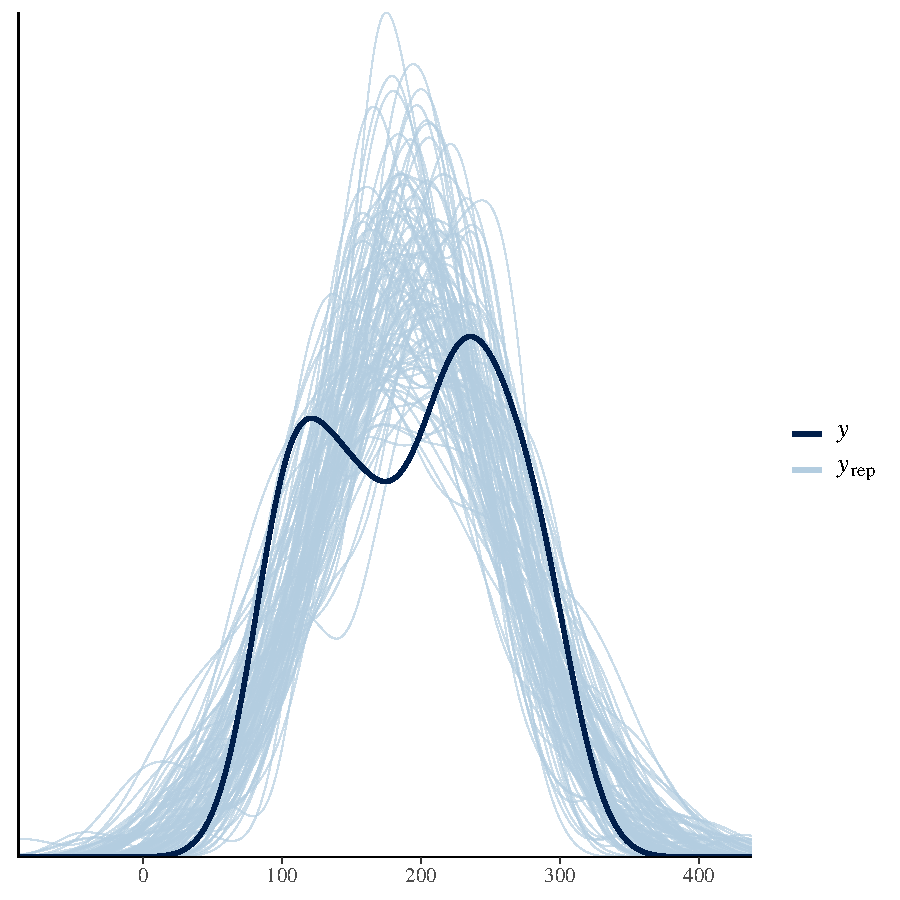
\includegraphics[width = 0.8\textwidth]{pics/pp_check_FE_noGender.pdf}
    \caption{Output of the posterior predictive check for a model \textbf{without} the predictor \texttt{gender}}
    \label{fig:coefficients_table}
\end{figure}


The model overestimates the probability of very low and high pitch values, underestimates the probability of values that surround our two bumps and heavily overestimates the probability of values around 200 Hz.
Our earlier model which takes \texttt{gender} into account looks quite a bit better. While still showing much uncertainty surrounding the two bumps in the observed distribution, it clearly captures the evidence better. 

\begin{figure}[]
  \centering
    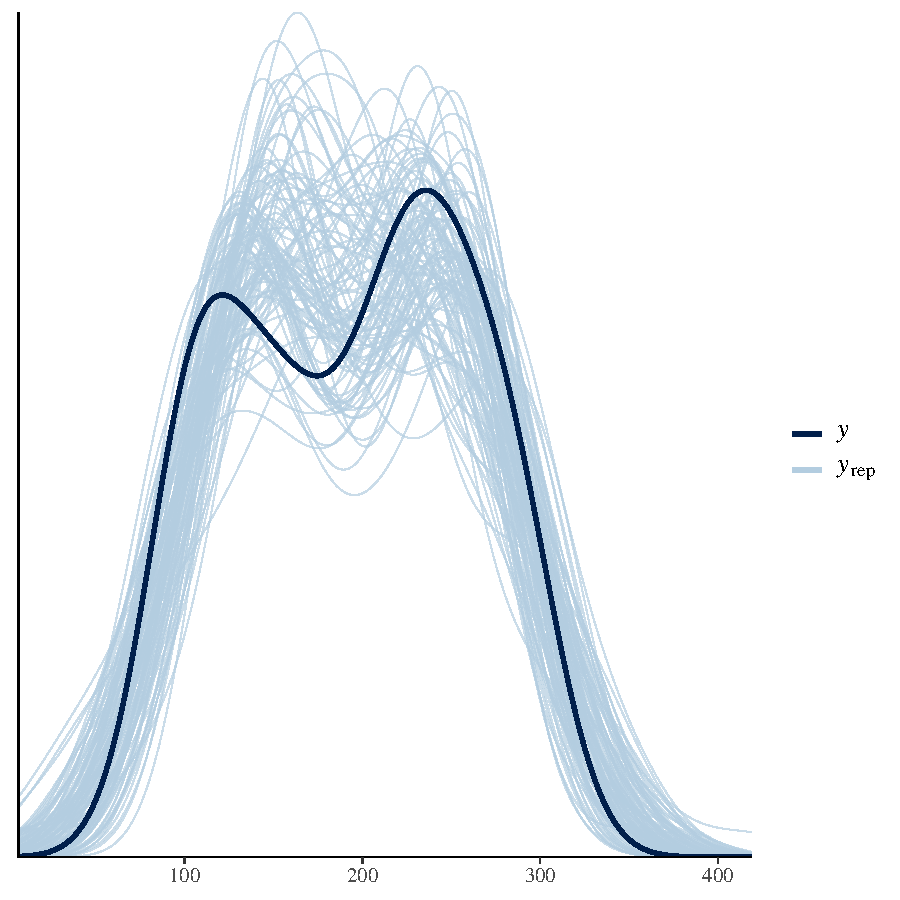
\includegraphics[width = 0.8\textwidth]{pics/pp_check_FE.pdf}
    \caption{Output of the posterior predictive check for a model with the predictor \texttt{gender}}
    \label{fig:coefficients_table}
\end{figure}


\section{Adding random effects}
In our experiment, we measured pitch multiple times for each subject (since they produced multiple sentences). We also have multiple measures for each sentence (as each sentence was produced by multiple speakers). A crucial assumption of linear regression models is the independence assumptions. Many before us have covered this aspect of linear models \citep[e.g.][]{Winter2013:Linear-models-a, clark1973language} so we won't discuss this important issue here in detail. In a nutshell, we need to inform our model about these dependencies between observations. The way we’re going to handle this is to add random effects to our model, just as we do in frequentists' frameworks. Random effects are additional parameters that our Bayesian model estimates.

Although the results look quite different, running hierarchical random effect models with \textrm{brms} is very similar to the look and feel of non-Bayesian approaches. Here is the function call to a model with the maximal random effect structure licensed by the design. We also defined regularizing priors for the intercept and skeptical priors for the predictor coefficients.
The outcome of this is model fit is shown below:

\begin{minipage}[]{1\textwidth}
\begin{lstlisting}[language=R]
# define priors
prior_MaxRE <- c(
  # define a regularizing prior for the intercept within the range of possible pitch values
  prior(normal(194, 66), class = Intercept),
  # define a skeptical prior for the relevant coefficients
  prior(normal(0, 50), class = b)
)

# model
model_MaxRE = brm(formula = pitch ~ gender * context +
	(1 + gender * context | sentence) +
	(1 + context | subject),
	prior = prior_MaxRE,
	data = politedata,
	control = list(adapt_delta = 0.99)
	)
\end{lstlisting}
\end{minipage}

\medskip

\begin{minipage}[]{1.5\textwidth}
\begin{rc}
Family: gaussian 
  Links: mu = identity; sigma = identity 
Formula: pitch ~ gender * context + (1 + gender * context | sentence) + (1 + context | subject) 
   Data: politedata (Number of observations: 83) 
Samples: 4 chains, each with iter = 2000; warmup = 1000; thin = 1;
         total post-warmup samples = 4000

Group-Level Effects: 
~sentence (Number of levels: 7) 
                                   Estimate Est.Error l-95% CI u-95% CI Eff.Sample Rhat
sd(Intercept)                         21.89     10.35     7.07    46.85       1701 1.00
sd(genderM)                           10.66      8.59     0.39    31.99       2163 1.00
sd(contextpol)                        15.23     11.51     0.67    42.78       1495 1.00
sd(genderM:contextpol)                16.52     12.69     0.72    47.94       1906 1.00
cor(Intercept,genderM)                -0.23      0.44    -0.89     0.69       3745 1.00
cor(Intercept,contextpol)              0.00      0.41    -0.75     0.78       3625 1.00
cor(genderM,contextpol)               -0.07      0.44    -0.83     0.75       2620 1.00
cor(Intercept,genderM:contextpol)     -0.10      0.43    -0.84     0.73       4391 1.00
cor(genderM,genderM:contextpol)       -0.04      0.45    -0.82     0.79       2741 1.00
cor(contextpol,genderM:contextpol)    -0.14      0.45    -0.87     0.74       2562 1.00

~subject (Number of levels: 6) 
                          Estimate Est.Error l-95% CI u-95% CI Eff.Sample Rhat
sd(Intercept)                41.86     21.82    16.02   100.10       1295 1.00
sd(contextpol)                9.15      9.11     0.30    32.92       2009 1.00
cor(Intercept,contextpol)    -0.00      0.58    -0.94     0.95       3461 1.00

Population-Level Effects: 
                   Estimate Est.Error l-95% CI u-95% CI Eff.Sample Rhat
Intercept            238.25     26.09   180.41   282.88       1255 1.00
genderM              -79.10     34.17  -134.89    -0.44       1188 1.01
contextpol           -24.30     12.02   -47.03     0.39       2229 1.00
genderM:contextpol    11.13     16.28   -22.13    43.42       1820 1.00

Family Specific Parameters: 
      Estimate Est.Error l-95% CI u-95% CI Eff.Sample Rhat
sigma    25.00      2.36    20.83    30.02       3124 1.00

Samples were drawn using sampling(NUTS). For each parameter, Eff.Sample 
is a crude measure of effective sample size, and Rhat is the potential 
scale reduction factor on split chains (at convergence, Rhat = 1).
\end{rc}
\end{minipage}

The lines 29--34 again give the estimates of the fixed-effects coefficients. The mean estimates look very similar to the ones that we obtained in the fixed-effect only model above. However, not surprisingly, our uncertainty surrounding these estimates is larger.  
We now also get information about the parameters implied by the specified random effect
structure. Lines 9--21 cover the by-sentence random effects, lines 23--27 cover the by-subject
random effects.

To check the probability of our hypotheses of interest, we can use the \texttt{faintr} package again:

\medskip

\begin{minipage}[]{\textwidth}
\begin{rc}
> get_posterior_beliefs_about_hypotheses_new(model_MaxRE)
# A tibble: 3 x 2
  hypothesis                      probability
  <chr>                                 <dbl>
1 Female-polite < Female-informal       0.974
2 Male-polite < Male-informal           0.853
3 Male-informal < Female-polite         0.918
\end{rc}
\end{minipage}

When we compare these values to the simpler model above, we can see that our evidence for our hypotheses is a little bit weaker for the maximal random effect model. This is not surprising because the simpler model assumed independence where there was none and therefore underestimated the variance. This is particularly noteworthy for H3. Before, we were certain that H3 was true (the posteriors suggested a probability of 1).

\section{Reporting the results}
How do we report our analysis and our results in a Bayesian framework? There are as many ways to write up your analysis as there are authors. The following suggestion is one way to do it. 

\paragraph{Description of analysis}  
We fitted Bayesian hierarchical linear models to pitch values as a function of \texttt{gender}, and \texttt{context} and their two-way interaction, using the Stan modeling language \citep{carpenter2016stan} and the package \emph{brms} \citep{buerkner2016brms}.
The models included maximal random-effect structures justified by the design, allowing the predictors of interest and their interactions to vary by participants (\texttt{context}) and sentences (\textsc{gender}, \textsc{context}).
We used a regularizing Gaussian prior for the intercept defined centered around the mean of the observation with  \(\sigma = 66\). We used weakly informative Gaussian priors centered around zero with \(\sigma = 50\) for all population-level regression coefficients.  Four sampling chains with 2000 iterations each were run for each model, with a warm-up period of 1000 iterations. 
For all relevant predictor levels and differences between them, we report 95\% credible
intervals (CIs) and the posterior probability that a parameter $\beta$ is smaller than zero $P(\beta < 0)$. A 95\% credible interval demarcates the range of values that comprise 95\% of probability density or mass of our posterior beliefs. We judge there to be \emph{compelling evidence
} for an effect if zero is (by a reasonably clear margin) not included in the 95\% CI and $P(\|beta| < 0)$ is close to one.

\paragraph{Description of results}  
\tr{here we need the estimates of each level for our convenient data report, right? we havent done that above. Ideas?}


\section{Further reading}
e.g. Bayes factor





\printbibliography[heading=bibintoc]

\end{document}
